\subsection{Byggnadsskal - väggar och tak}

%Definition av h-värde och U-värde

\frame{
       \frametitle{Några definitioner}
        \begin{align*}
        Q &= U\Delta T \\
        Q &= h(T-T_\infty)
        \end{align*}
        \begin{center}
          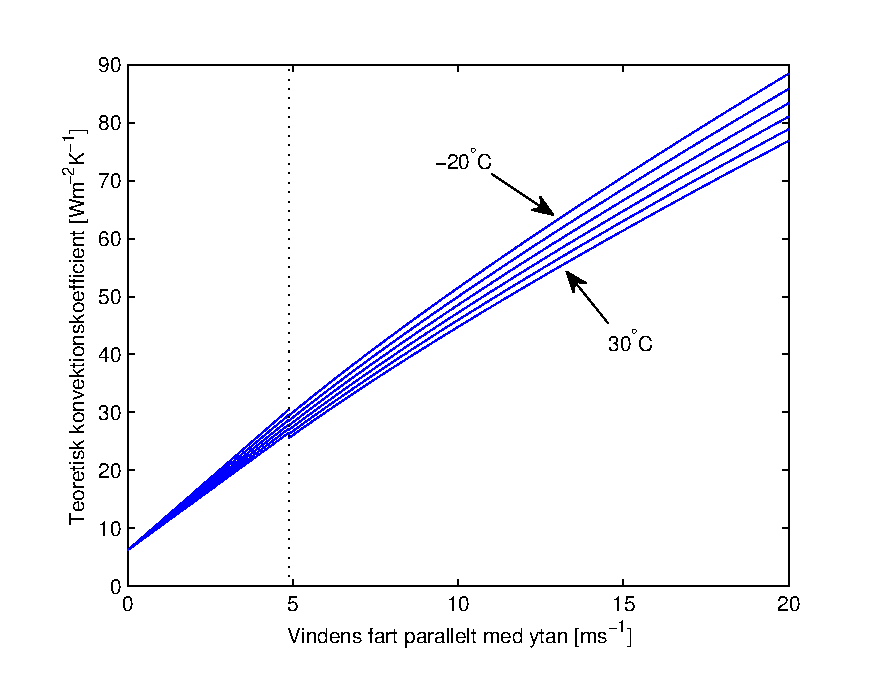
\includegraphics[scale=0.5]{../report/images/hvalues.eps}
        \end{center}
}


%Data för huset

\frame{
       \frametitle{Parametrar för huset}

       \begin{figure}
         \begin{subfigure}[b]{0.48\textwidth}
           \centering
           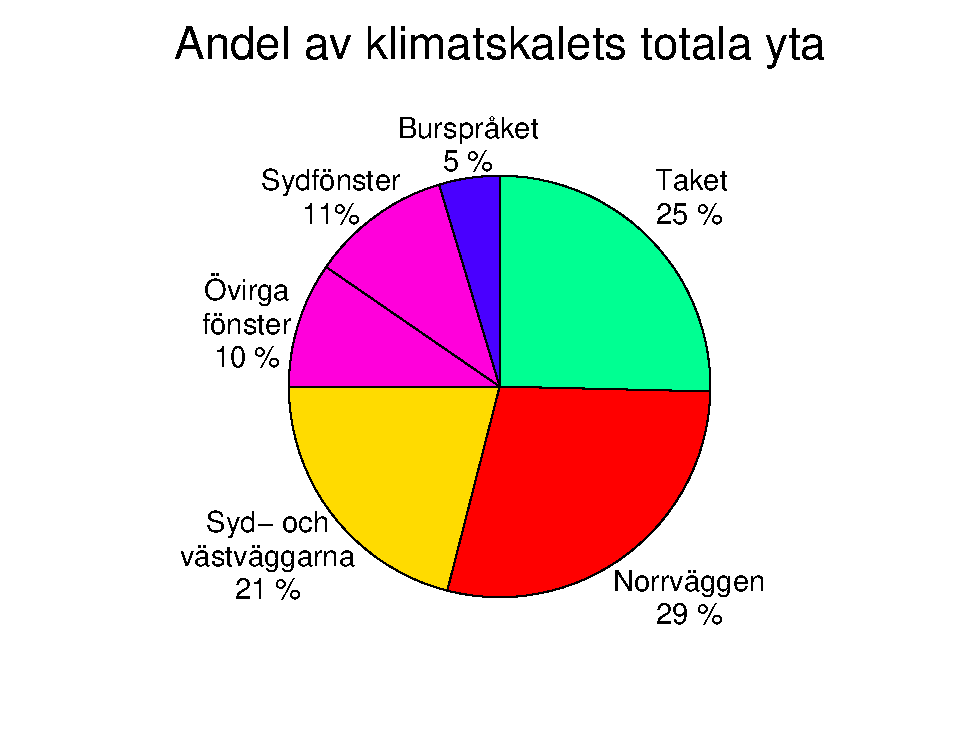
\includegraphics[width=\textwidth]{images/areor_klimatskal.eps}
         \end{subfigure}
         \begin{subfigure}[b]{0.48\textwidth}
           \centering
           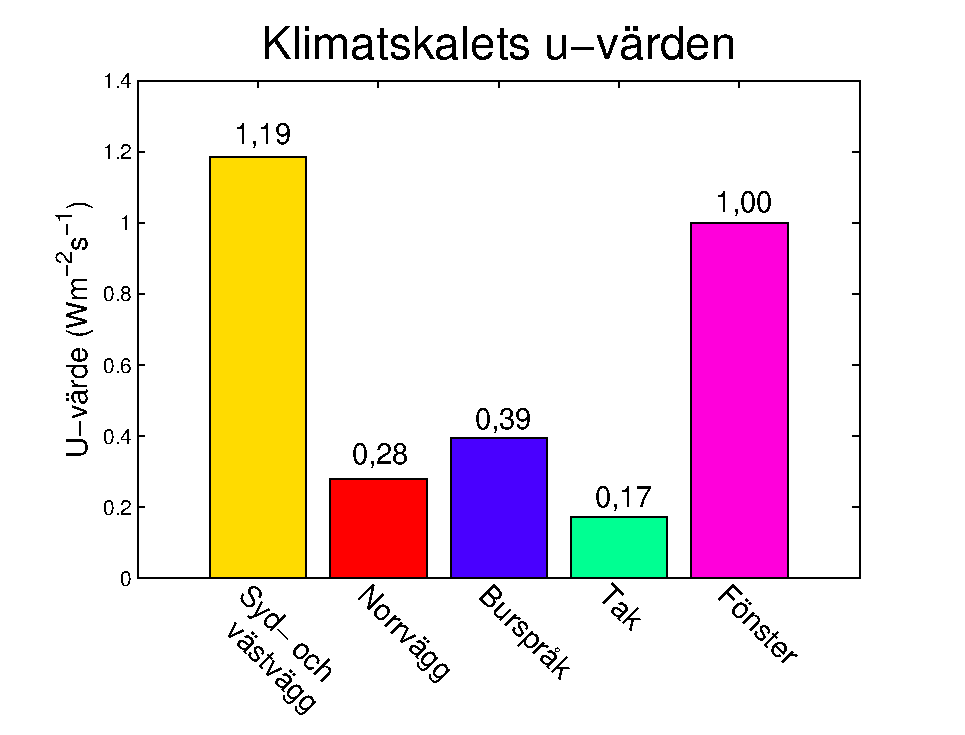
\includegraphics[width=\textwidth]{images/uvalue.eps}
         \end{subfigure}
       \end{figure}
}

\begin{frame}{Energiflöden, väggar och tak\\En klar decemberdag}
 
\begin{figure}
        \begin{subfigure}[b]{0.48\textwidth}
                \centering
                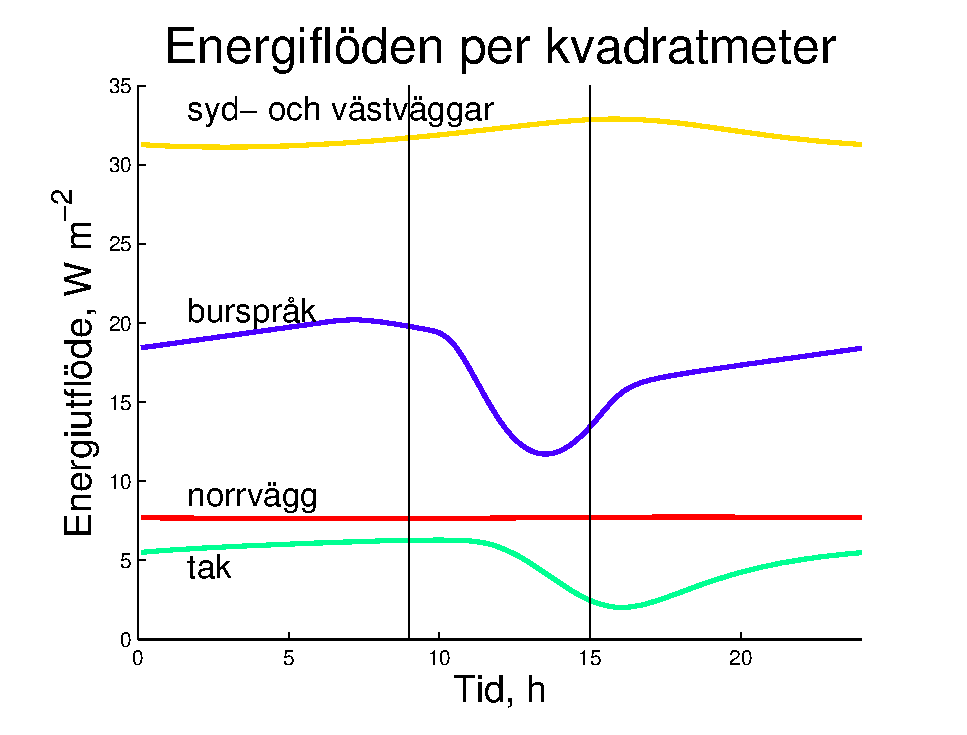
\includegraphics[width=\textwidth]{images/walls1.eps}
        \end{subfigure}
	\uncover<2>{
        \begin{subfigure}[b]{0.48\textwidth}
                \centering
                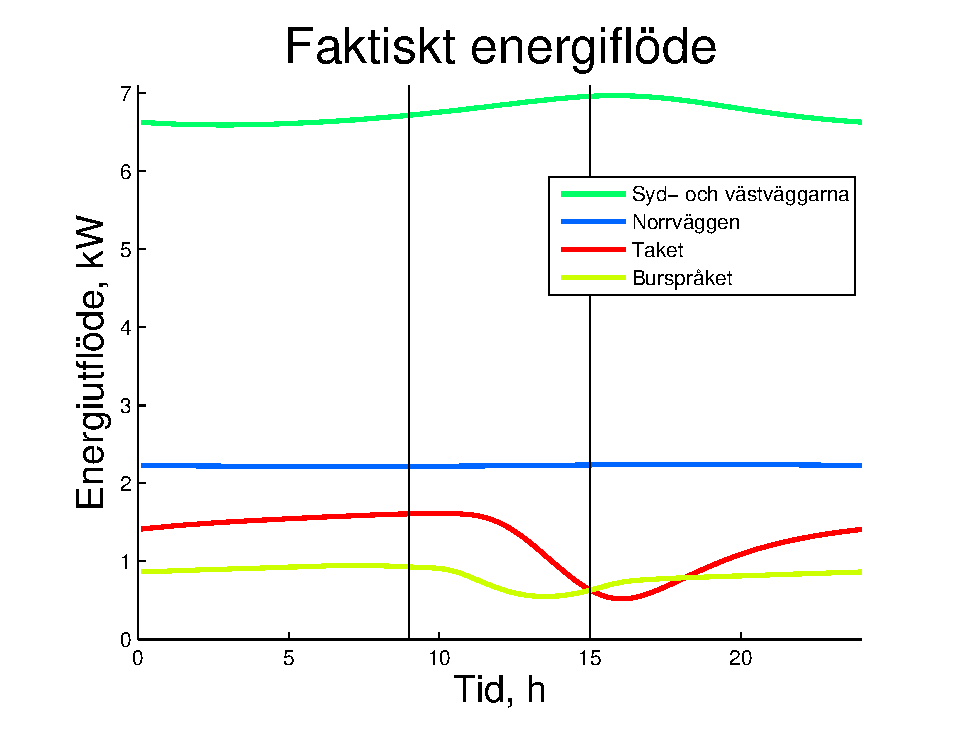
\includegraphics[width=\textwidth]{images/walls2.eps}
        \end{subfigure}
        }
\end{figure}


\end{frame}

